\documentclass[3p, sort&compress]{elsarticle}
\usepackage{amsmath}
\usepackage{amssymb}
\usepackage{amsthm}
\usepackage{amsfonts}
\usepackage{amsbsy}
\usepackage{amstext}
\usepackage{amsfonts}
\usepackage{amstext}
\usepackage{mathrsfs}
\usepackage{graphpap}
\usepackage{graphics,graphicx}
\usepackage[utf8]{inputenc}
\usepackage{subcaption}
\usepackage{multicol}
\usepackage{booktabs}
\usepackage{array}
\usepackage{siunitx}
\usepackage{hyperref}
\usepackage[section]{placeins}
\usepackage{xargs}
\usepackage[pdftex,dvipsnames]{xcolor}
\usepackage[colorinlistoftodos,prependcaption,textsize=tiny]{todonotes}
\graphicspath{{./plotly_chart_studio_figures/}}
\graphicspath{{./figures/}}
%
%
\newcommandx{\unsure}[2][1=]{%
    \todo[
        linecolor=red,
        backgroundcolor=red!25,
        bordercolor=red, #1]{#2}
}%
\newcommandx{\change}[2][1=]{%
    \todo[
        linecolor=blue,
        backgroundcolor=blue!25,
        bordercolor=blue, #1]{#2}
}
\newcommandx{\info}[2][1=]{%
    \todo[
        linecolor=OliveGreen,
        backgroundcolor=OliveGreen!25,
        bordercolor=OliveGreen, #1]{#2}
}
\newcommandx{\improvement}[2][1=]{
    \todo[linecolor=Plum,
        backgroundcolor=Plum!25,
        bordercolor=Plum,#1]{#2}
}
\newcommandx{\thiswillnotshow}[2][1=]{\todo[disable,#1]{#2}}
\hypersetup{colorlinks = true, allcolors = blue}
\usepackage[nameinlink,noabbrev]{cleveref}
\newcommand{\R}{\mathbb{R}}
\newcommand{\e}{\varepsilon}
\newcommand{\f}{\mathfrak{F}}
\newcommand{\Q}{\mathbb{Q}}
\newcommand{\N}{\mathbb{N}}
\newtheorem{teor}{Theorem}
\newtheorem{lemma}{Lemma}
\usepackage[toc,page]{appendix}
%
%
\begin{document}
    \begin{frontmatter}
        \title{
            Optimal vaccination preventive policies for COVID-19\\
        }
        \author[add:conacyt_unison]{%
            Sa\'ul D\'iaz-Infante%
            \corref{corresponding_author}%
        }%
        \ead{saul.diazinfante@unison.mx}
        \address[add:conacyt_unison]{
            CONACYT-Universidad de Sonora, Departamento de Matem\'aticas,
            Blvd. Luis Encinas y Rosales S/N,
            Hermosillo, Sonora, M\'exico, C.P. 83000.
        }
        %%%%%%%%%%%%%%%%%%%%%%%%%%%%%%%%%%%%%%%%%%%%%%%%%%%%%%%%%%%%%%%%%
        \author[add:unison]%
        {Manuel Adrian Acu\~na-Zegarra}
        \ead{adrian.acuna@unison.mx}
        \address[add:unison]{
            Departamento de Matem\'aticas, Universidad de Sonora,
            Blvd. Luis Encinas y Rosales S/N,
            Hermosillo, Sonora, M\'exico, C.P. 83000.
        }
        %%%%%%%%%%%%%%%%%%%%%%%%%%%%%%%%%%%%%%%%%%%%%%%%%%%%%%%%%%%%%%%%%
        \author[add:itson]%
            {David Baca-Carrasco}
            \ead{david.baca@itson.edu.mx}
        \address[add:itson]{
                Departamento de Matem\'aticas, Instituto Tecnol\'ogico de
                Sonora, 5 de Febrero 818 Sur, Colonia Centro, Ciudad
                Obregón,
                Sonora, M\'exico, C.P. 85000.
        }
        \author[add:unison]%
        {Daniel Olmos-Liceaga}
        \ead{daniel.olmos@unison.mx}
    \cortext[corresponding_author]{Corresponding author}
    \begin{keyword}
        Optimal Control, COVAX
        Vaccination, COVID-19.
    \end{keyword}
    \begin{abstract}
        BACKGROUND
        At the date, Europe and North America experiments the second wave of
        COVID-19 causing more than \num{1200000} deaths worldwide.
        Humanity lacks of successful treatment and the only plausible solution
        is an effective vaccine. Currently,four are in final phase three trials.
        If third stage trial results favorable, Pharmaceutics firms
        estimate big scale production of its vaccine candidates around
        first 2021  quarter.
        However, determine the vaccine efficacy, induced immunity response
        among other essential parameters still are under study and subject to
        uncertainty. In fact, is possible that
        first  vaccines will not be fully protective.
        Instead they may reduce the severity of illness, reducing
        hospitalization and death cases.
        Further, logistic supply, economical and political implications
        impose a set of great challenges to develop vaccination policies.
        PROBEM SETUP
        For this reason, health decision makers requires tools to evaluate
        hypothetical scenarios.
        FINDINGS
        Our contribution partially answers
        important modeling questions regarding to WHO Strategic
        Advisory Group of Experts (SAGE) on
        Immunization Working Group on COVID-19 Vaccines.

        Our results suggest that optimal control theory could be an option
        tool to develop  vaccination policies that satisfies important
        constrains as coverage horizon time supply restriction. We also report
        here simulation of vaccination polices with vaccine parameters reported
        by the most promising alternatives.

        COVID-19, which includes vaccination dynamics. We apply optimal control
        theory to propose optimal vaccine strategies that minimize DALYs.
        Additionally, we analyze the vaccination reproductive number around the
        basic reproductive number and the vaccination profile (coverage,
        efficacy,
        horizon time, and vaccination rate). Due to the uncertainty about the
        profile vaccine, our results explore some scenarios regarding efficacy,
        coverage, induced immunity by vaccination, and natural immunity. Here,
        we
        observe that: i) there are strategies that reduce DALYs and cumulative
        deaths at the horizon time compare to its counterpart with constant
        vaccination; ii) it is necessary information about vaccine efficacy to
        design optimal strategies, and iii) ...
    \end{abstract}
    \journal{Mathematical Biosciences}
\end{frontmatter}
%
    \section{Introduction}
        In late December 2019, a new virus's appearance is reported in Wuhan City,
Hubei Province, China. Called SARS-CoV2, it is the virus that causes the 2019
corona virus disease (COVID-19) and that, very quickly since its appearance,
has spread throughout much of the world, causing severe problems to health
systems of all the countries in which it is present \cite{Who12020}. On March
11, 2020, the World Health Organization declared the epidemic by COVID-19 as a
pandemic when there were around 118,000 cases distributed in 114 countries, and
approximately 4,291 deaths \cite{Who512020}. In Latin America, the first
detected case of COVID-19 occurred in Brazil on February 26, and in Mexico, the
first case was reported on February 27, quickly spreading throughout the
country \cite{Ajrm2020,Acuna2020}.

Due to the absence of successful treatment and vaccines,
several non-pharmaceutical interventions (NPIs) have been implemented in all the
countries where the disease is present, with quarantine, isolation, and social
distancing being the main ones \cite{Wilder2020,Guner2020,Liu2020_2}. Despite
the measures that different governments have taken to mitigate the epidemic, it
has not been controlled in most places, which may be due to the relaxation of
mitigation measures. At the date of writing this work, the upturn or regrowth
in the number of cases in some countries around the world has been observed. In
some places, this behavior is referred to as "second wave". On the other hand,
since the new coronavirus appearance, the international scientific community
has been working to understand the virus nature. They mainly focus on the
spreading mechanisms between individuals, and developing vaccines and
treatments to reduce the number of infections and fatality cases. To get a
clearer understanding of different vaccination strategies and their
consequences on the number of infected individuals, mathematical models have
taken a leading role.

    The use of various mathematical tools such as SIR and SEIR models has
helped to  describe epidemics properties around the globe. These models have
been used to estimate the basic reproductive number associated with the disease
and also different parameters involved in its spread
\cite{Wang2020,Liu2020,Sarkar2020,Hong2020}. Another use of this kind of model
has been addressed to propose and evaluate the effect of various control
measures classified as NPIs
\cite{Acuna2020,Marimuthu2020,Liu2020,Shaikh2020,DeVisscher2020}.

    Currently, vaccine development for COVID-19 is at an advanced stage. It is
believed that their distribution will begin in early 2021. However, we
consider that, in addition to the vaccine's existence, it is necessary to
have a good vaccination strategy. A widely used tool to address this
question is the optimal control theory. This mathematical tool is useful to
propose scenarios in which the vaccine's application minimizes the damage
caused by the disease and its application cost. Some results about it have
been applied to control other diseases for humans and animals
\cite{Asano2008,Rodrigues2014,Tchuenche2011,Malik2016,Jaberi2014}. Optimal
control theory has also been used in COVID-19 studies. Most efforts have
been invested in finding optimal strategies to evaluate the impact of
non-pharmaceutical interventions
\cite{Madubueze2020,Perkins2020,Ullah2020}. Optimal control strategies have
also being considered in vaccination \cite{Barbosa2020}. In this work, the
authors took their optimization based on a basic compartmental model for
COVID-19. In their model, deaths due to disease are not considered and
vaccination is applied only to susceptible individuals.  \unsure{NO SE VE
    LA DIFERENCIA RESPECTO A NUESTRO TRABAJO, EL QUE NO CONSIDEREN MUERTE NO LO
    HACE TAN DIFERENTE. RECUERDO QUE SAÚL MENCIONÓ ALGO SOBRE QUE LA FORMA DE
    HACER CONTROL ES DISTINTA. O DE PLANO NO HAY? JAJA....Ohh pues...dejame
    ser! estoy en eso!}

In this work, we present a mathematical model to describe the transmission and some vaccination dynamics of COVID-19. Mainly, we focus on using optimal control theory to obtain vaccination strategies in a homogeneous population. Our main objective is to minimize the disability-adjusted life year (DALY) \cite{WhoDALY}. This quantity is used by the World Health Organization (WHO) to quantify the burden of disease from mortality and morbidity, which is given by the sum of the years of life lost (YLL) and years lost due to disability (YLD). This work's objective is framed within the context of the WHO strategic advisory group of experts (SAGE) on immunization working group on COVID-19 vaccines \cite{sage2020}.

Development of COVID-19 vaccines is a major challenge these days. Some research efforts in this direction can be found in \cite{Belete2020,Kaur2020}. In Mexico, some of the considered vaccines to be applied to the population are Adenovirus Type 5 Vector (Ad5-nCoV) by Cansino Biologics, AZD1222 by AstraZeneca and BNT162b2 by Pfizer and BioNTech. At the current date, these and other vaccines are on the testing phase (phase 3) and there are still some questions about the efficacy of the vaccines. In the United States, an appropriate vaccine to be applied needs to show firm evidence that it protects at least half of those inoculated \cite{Shah2020}. At this stage, there are no conclusive results about the efficacy of the vaccines. Also, current work is the immunity time the vaccines will provide to people.

Our work is divided into the following sections. In Section 2, we present our mathematical model, which includes preventive vaccine dynamics. Section 3 includes an analysis of the vaccination reproductive number. Section 4 presents our numerical results regarding optimal vaccination policies. It is important to stress that, with the objective of study COVID-19 dynamics in a specific city and have a set of baseline parameters values, we used the Mexico City plus Mexico state COVID-19 data to estimate some proposed model parameters. We end this work with a conclusions and discussions section.
    \section{Mathematical model formulation}
        
In this section, we formulate our baseline mathematical model,
which additionally to the transmission dynamics, includes vaccination.
In order to build our  model, we follow the classical Kermack-McKendrick
approach. \Cref{Fig:SchemeModel} shows the compartmental diagram of
our mathematical model.
\begin{figure*}[tbh]
    \centering
    \includegraphics[scale = 1]{SchemeModel_0211_v3.pdf}
    \caption{%
        Compartmental diagram of COVID-19 transmission dynamics which
        including vaccination dynamics. Here, there are seven different classes:
        Susceptible $(S)$, exposed $(E)$, symptomatic infected $(I_S)$, asymptomatic
        infected $(I_A)$, recovered $(R)$, death $(D)$ and vaccinated $(V)$
        individuals. It is important to mention that $I_{S}$ represents the
        proportion of symptomatic individuals who will later report
        to some health medical center.}
    \label{Fig:SchemeModel}
\end{figure*}

Information about reinfection dynamics on COVID-19
disease is unclear to date. However, to explore some scenarios related
to this dynamic, we assume that reinfection is possible after a period
of time. On the other hand, we model the vaccination process considering
some assumptions: i) Vaccination is applied to all the alive individuals
except those in the symptomatic class. In this situation, vaccines are
applied indiscriminately over individuals on the $S$, $E$, $I_A$, and
$R$ classes; ii) the vaccine has preventive nature, that is, only
reflected in the susceptible individuals $(S)$; iii) people will only get
one vaccine during the campaign, and iv) vaccines do not necessarily have
a hundred percent of effectivity, which implies that some vaccinated people
can get the disease. We denote the effectivity rate by $\epsilon$.
Based on these assumptions our model becomes
\begin{equation}\label{model1}
    \begin{aligned}
        S'(t) &= \mu \bar{N}-\frac{\beta_S I_S +
            \beta_AI_A}{\bar{N}}S - (\mu+\lambda_V)S +
        \delta_V V+ \delta_R R
        \\
        E'(t) &= \frac{\beta_S I_S + \beta_AI_A}{\bar{N}}S+
        (1-\epsilon) \frac{\beta_S I_S+\beta_AI_A}{\bar{N}}V-(\mu+\delta_E) E
        \\
        I'_S(t) &=
        p \delta_E E-(\mu+\alpha_S) I_S
        \\
        I'_A(t) &= (1-p) \delta_E E-(\mu+\alpha_A) I_A
        \\
        R'(t)&= (1-\theta) \alpha_S I_S +
        \alpha_A I_A-(\mu+\delta_R) R
        \\
        D'(t) &= \theta \alpha_S I_S
        \\
        V'(t) &= \lambda_V S-(1-\epsilon)
        \frac{\beta_S I_S + \beta_AI_A}{\bar{N}}V - (\mu+\delta_V) V
        \\
    \end{aligned}
\end{equation}
%
where $\bar{N}(t)=S(t)+E(t)+I_S(t)+I_A(t)+R(t)+V(t)$ and
$N=\bar{N}+D$. Additionally, we include the equations
\begin{equation}
    \label{eqn:model1_counters}
    \begin{aligned}
        X'(t) &=
        \lambda_V(S + E + I_A + R)
        \\
        Y'_{I_S}(t) &=p
        \delta_E E,
    \end{aligned}
\end{equation}
where $X(t)$ and $Y_{I_S}(t)$ represent the cumulative doses at time $t$,
and the cumulative incidence at time $t$, respectively.
Parameters description of system in \Cref{model1} is provided
in \Cref{table:parametermodel}.

\begin{table*}[tbh]
    \centering
    \begin{tabular}{cl}
        \toprule
        Parameter & Description
        \\
        \midrule
        $\mu$ &  Natural death rate
        \\
        $\beta_S$ & Infection rate between susceptible and symptomatic infected
        \\
        $\beta_A$ & Infection rate between susceptible and asymptomatic infected
        \\
        $\lambda_V$ & Vaccination rate
        \\
        $\delta_{V}^{-1}$ & Immunity average time by vaccination
        \\
        $\epsilon$ &  Vaccine efficacy
        \\
        $\delta_{E}^{-1}$ & Average time of the incubation period \\
        $p$ & Proportion of symptomatic individuals  \\
        $\alpha_{S}^{-1}$ &  Average output time of symptomatic
        individuals due to death or recovery  \\
        $\theta$ & Proportion of symptomatic individuals who die due to
        the disease \\
        $\alpha_{A}^{-1}$
        & Recovery average time of asymptomatic individuals
        \\
        $\delta_{R}^{-1}$
        &  Immunity average time by disease
        \\
        \bottomrule
    \end{tabular}
    \caption{Parameters definition of system in \Cref{model1}.}
    \label{table:parametermodel}
\end{table*}

\subsection{Baseline parameters value and initial conditions}
It is now necessary to define a set of baseline parameter
values to explore some scenarios of interest. In the present work,
we consider Mexico City plus Mexico state as our study region and use
COVID-19 data to estimate some parameter values. We follow a Bayesian
approach to address this problem. We use a negative binomial
distribution as an observation model, in which the mean parameter
is given by
\begin{equation*}\label{incidence}
    \begin{aligned}
        I_{SA}(k) = Y_{I_S}(k) - Y_{I_S}(k-1)=\int_{k-1}^k p\delta_EE dt,
    \end{aligned}
\end{equation*}
where $I_{SA}(k)$ represents the incidence per day of
infected symptomatic individuals at the $k-th$ day.
The parameter estimation splits into two-stage:
before and after mitigation measures were implemented,
and we only focus on the early phase of the COVID-19 outbreak.
\Cref{Fig:fittingcurve} shows fitting curves with their respective
confidence bands for both stages. Here, we observe that our estimations
follow the growth profile of the epidemic curve. For more information about
the parameter estimation process, see \Cref{App:Parameter_Est}.
\Cref{table_icparam4} resume our parameter calibration.
%
\begin{figure*}[tbh]
    \centering
    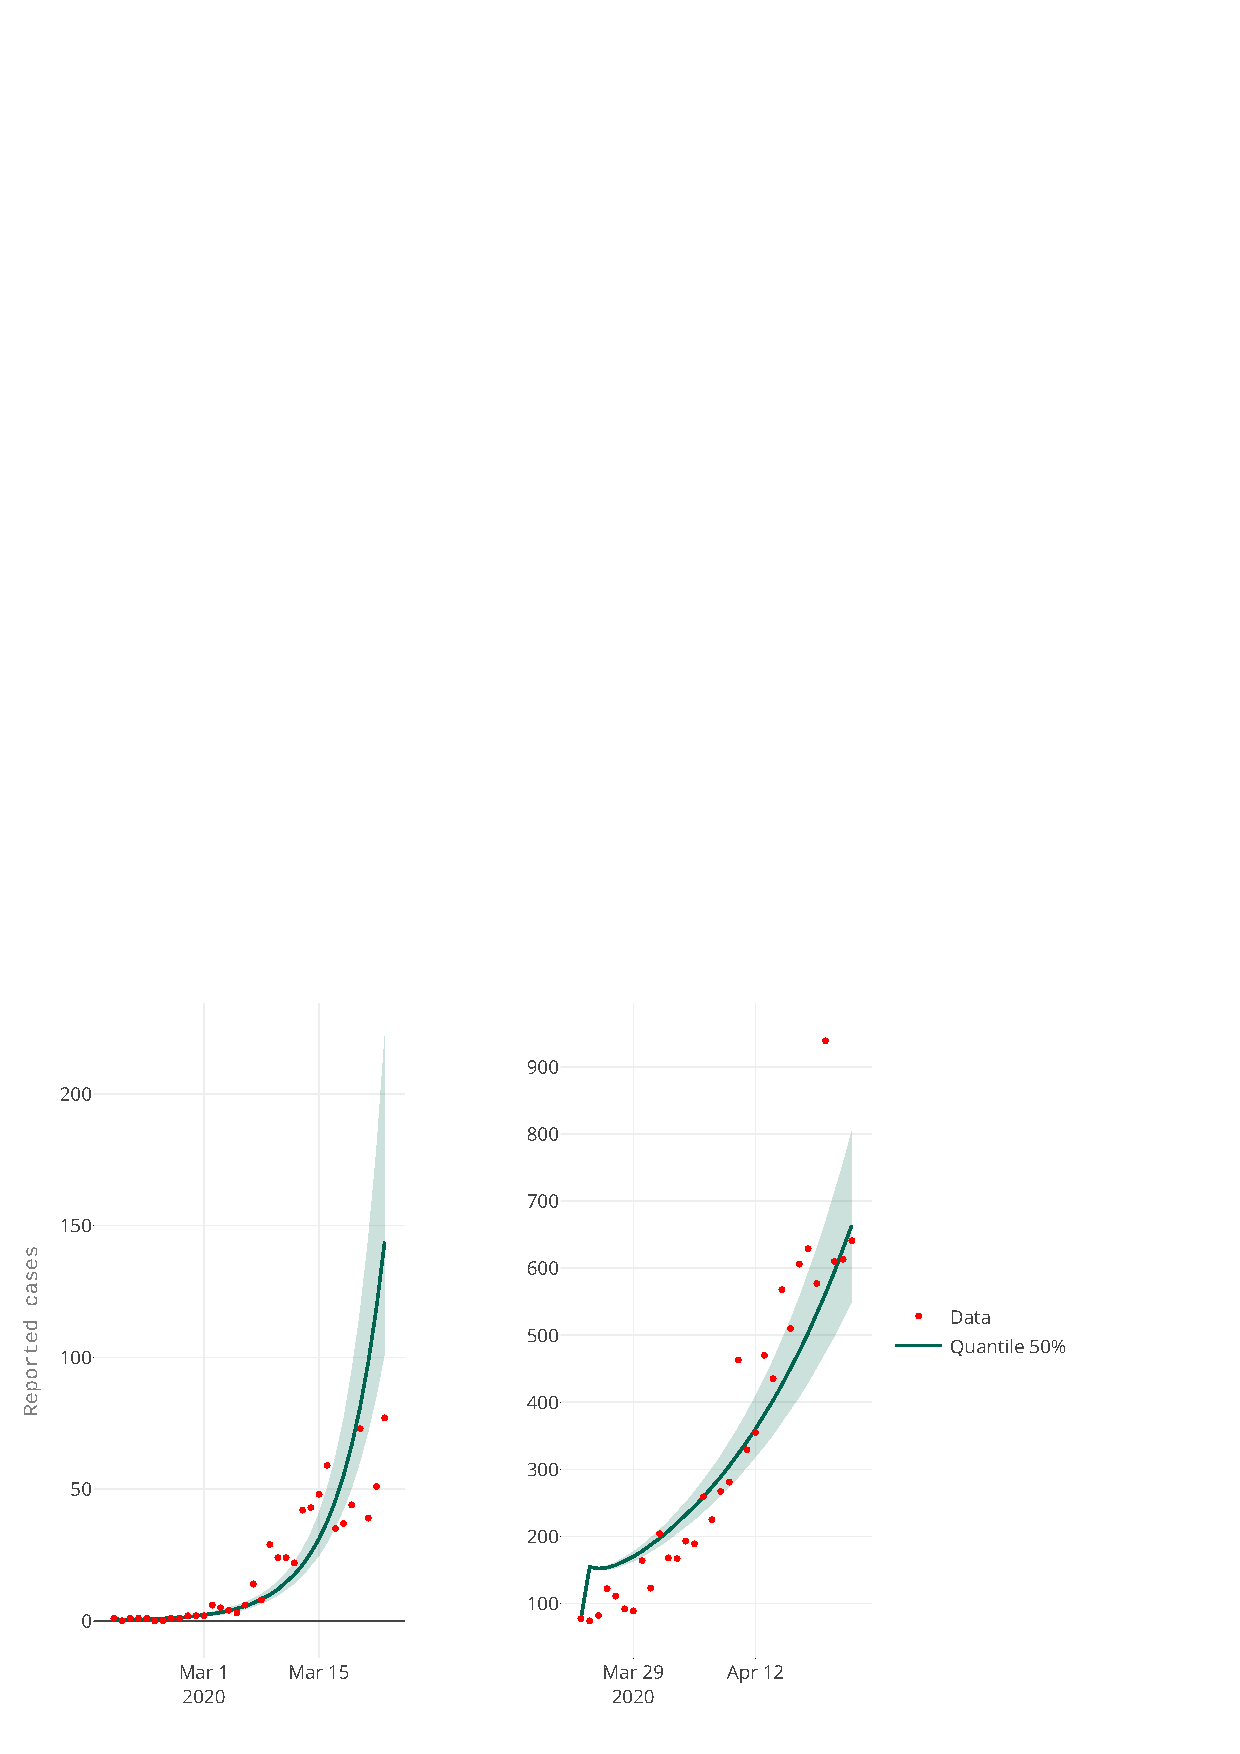
\includegraphics[scale=0.6, keepaspectratio]{FittingCurves.png}
    \caption{
        Fitting curves for the early phase of the COVID-19
        outbreak in Mexico City plus Mexico state.
        (A) Outbreak from February 19 to March 23, 2020.
        (B) Outbreak from March 23 to April 23, 2020.
        Reported data are shown in blue points, solid red line
        denote quantile 50 of all solutions
    }
    \label{Fig:fittingcurve}
\end{figure*}
%
\begin{table}[bth]
    \begin{center}
        \begin{tabular}{rl}
            \toprule
            Parameter & 95\% Confidence Interval
            \\
            \midrule
            $\beta_S$ & $[\num{0.2483712}, \num{0.48720714}]$ \\
            $\beta_A$ & $[\num{0.1851696}, \num{0.32181249}]$ \\
            $p$       & $[\num{0.061}, \num{0.2206}]$ \\
            $R_0$     & $[\num{1.702}, \num{1.887}]$\\
            \bottomrule
        \end{tabular}
        \caption{%
            Confidence interval for some parameters of system in
            \Cref{model1}, and for the basic reproductive number
            $(R_0)$.
        }\label{table_icparam4}
    \end{center}
\end{table}
%
On the other hand, since it is unclear when the vaccines will be available,
then we assume that our scenarios start on the growth stage of a second
outbreak (see \Cref{Fig:initial_conditions}) with the objective of starting
under a plausible scenario. Thus, for numerical results, initial conditions
normalized with total population
$N = \num{26446435}$, result
$S(0) = \num{0.463606046009872}$,
$E(0) = \num{0.00067033}$,
$I_S(0) = \num{0.00009283}$,
$I_A(0) = \num{0.00120986}$,
$R(0) = \num{0.532520194}$,
$D(0) = \num{0.00190074}$,
$V(0) = 0$, $X(0) = 0$, and
$Y_{I_{S}}(0) = \num{0.12258164}$.
\begin{figure*}[tbh]
    \centering
    \includegraphics[scale=0.6, keepaspectratio]{Is_dynamics.png}
    \caption{
        Dynamics of the symptomatic individuals. Black arrow indicates
        the outbreak stage in which we start our simulations.}
    \label{Fig:initial_conditions}
\end{figure*}
    \section{Model Analysis}
        %\textbf{[David]}
        In this section, we use the estimated parameters from the previous section
to analyze model in \Cref{model1} and the effect of the vaccine. Some
plausible scenarios are presented, depending on the effectiveness of the
vaccine,  as well as the rate of vaccination.

In the first instance, it has been shown that the interest region of the
state variables of the system is positively invariant and the proof can be
found in \Cref{apx:positivity_invariace}.

Now, an important concept in the analysis of the spread of diseases is the
basic reproductive number, defined as the number of secondary infections
produced by a typical infected individual, throughout his infectious period,
when in contact with a totally susceptible population. Following ideas of
\cite{Van2002}, the basic reproduction number for system in \Cref{model1} is (see
\Cref{apx:positivity_invariace})
\begin{equation}\label{Rv}
    \begin{aligned}
        R_{V} &=
            R_S + R_A
        \\
        R_S &=
            \frac{
                p \beta_S \delta_E
                (\mu + \delta_V + (1 - \epsilon)
                \lambda_V)
            }{
                (\mu + \delta_E)
                (\mu + \delta_V + \lambda_V)
                (\mu + \alpha_S)
            }
            \\
        R_A &=
            \frac{
                (1-p) \beta_A \delta_E
                (\mu + \delta_V + (1-\epsilon) \lambda_V)
            }{
                (\mu + \delta_E)
                (\mu + \delta_V + \lambda_V)
                (\mu + \alpha_A )
            }.
    \end{aligned}
\end{equation}

Note that each sum of $ R_ {V} $ represents the contribution of the symptomatic and
asymptomatic infected, respectively, to the spread of the disease.
Following the ideas of Alexander et. al. \cite{Alexander2004},
expression for $R_V$ can be rewritten as%
\begin{equation}\label{Rv2}
    R_{V} = R_0 \left(1- \frac{\epsilon \lambda_V}{(\mu+\delta_V+\lambda_V)}\right)
\end{equation}
where
\begin{equation}\label{R0}
    R_0 = \frac{p\delta_E\beta_S}{(\mu+\delta_E)(\mu+\alpha_S)} +
    \frac{(1-p) \delta_E \beta_A}{(\mu+\delta_E)(\mu + \alpha_A)}
\end{equation}
is the basic reproduction number of the system without vaccine.
Note that
$\left(1- \frac{\epsilon \lambda_V}{(\mu+\delta_V+\lambda_V)}\right)<1$. Therefore, this
factor, which enclose the  parameters corresponding to the application of the vaccine, will
allow us to modulate the value of $ R_0 $. In the  first instance, if $ R_0 <1 $,
then $ R_V <1 $. But, if $ R_0> 1 $, we ask if the application of the vaccine can
lower $R_V$ value below 1. In this sense, it is easy to prove that, if
\begin{equation}\label{condition1}
    \lambda_V>\frac{(R_0-1)(\mu+\delta_V)}{(\epsilon-1)R_0+1},
\end{equation}
%
for $\epsilon>1-(1/R_0)$, it is possible to reduce the value of $ R_V $ below one.
That is, there is a region in the parameter space in which it is possible to reduce
the value of $ R_V $ below one, considering adequate efficacy, vaccination rate and
duration of the effect of the vaccine. However, if the Inequality
\eqref{condition1} is not satisfied, it will not be possible to reduce the value of
$ R_V $ below 1.

To illustrate the aforementioned, \Cref{R0-2D} shows the regions where it is possible to
reduce the value of $ R_V $. In this case, we set all the system parameters as given in
\Cref{tbl:fixed_parameters} and with $ \delta_V = 1/180 $, leaving $ \epsilon $ and $
\lambda_V $ free.
\begin{table}[h!]
    \begin{center}
        \begin{tabular}{rl}
            \toprule
            Parameter & Value
            \\
            \midrule
            $\beta_S$ & $ \num{0.363282}$
            \\
            $\beta_A$ & $\num{0.251521}$
            \\
            $\alpha_{S}$  & $\num{0.0925069}$
            \\
            $\alpha_{A}$ & $\num{0.167504}$
            \\
            $\delta_{E}$ & $\num{0.196078}$
            \\
            $\delta_{R}$ & $\num{0.00273973}$
            \\
            $\mu$        & $\num{0.0000391389} $
            \\
            $\theta$        & $\num{0.11}$
            \\
            $p$        & $\num{0.1213} $
            \\
            \bottomrule
        \end{tabular}
        \caption{%
            Fixed parameters values of system in \Cref{model1}.
            The parameters corresponding to vaccination are
            established in each scenery studied.}
        \label{tbl:fixed_parameters}
    \end{center}
\end{table}
%
\begin{figure*}[tbh]
    \centering
    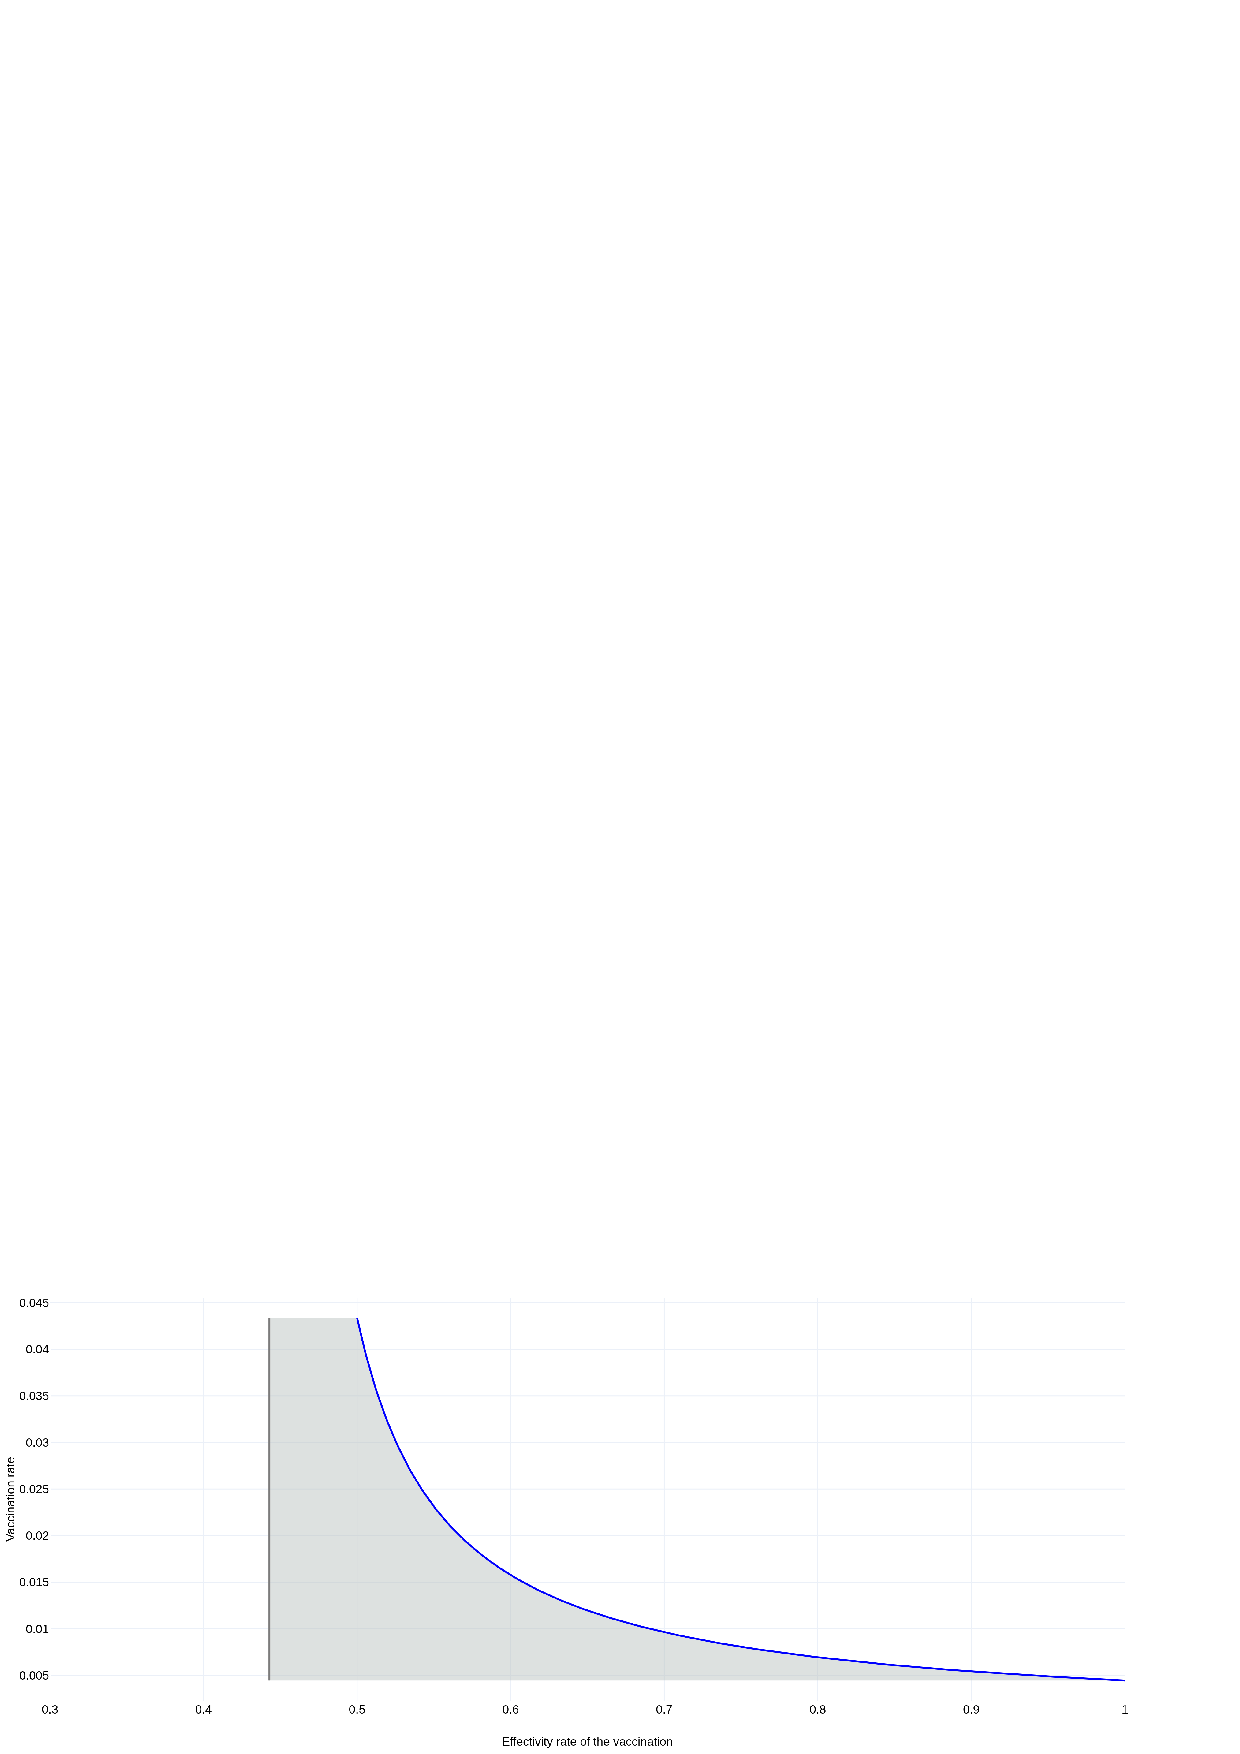
\includegraphics[scale=0.6]{R0-2D.png}
    \caption{
        Vaccine efficacy versus vaccination rate feasibility.
        In the shaded region $R_V>1 $ and in the white region $ R_V <1 $.
        Note that, for our scenario, with a $50$ percent vaccine effectiveness
        and an adequate vaccination rate, it is possible to reduce the $ R_V $
        value below one. The orange region is unfeasible.}
    \label{R0-2D}
\end{figure*}

\subsection{Baseline vaccination rate formulation}
Vaccination policies to reach a given coverage of a
certain percentage of the population in a given period is of great importance.
In this sense, we refer to this vaccination constant rate as the base vaccination
rate, denoted by $ \lambda_{Vbase}$.

Let $W(t)$ be the normalized unvaccinated population at time $t$, we consider
that at $t=0$ no person has been vaccinated, which implies $W(0)=1$.
Then, by assuming that we vaccinate individuals at a constant rate $\lambda_{Vbase}$
proportional to the actual population, we have that $W(t)$ satisfies the equation
$$
\dot{W}(t)=-\lambda_{Vbase} W(t)
\qquad \qquad \textrm{with} \qquad\qquad {W(0)=1}
$$
or $W(t)=e^{-\lambda_{Vbase}t}$. It implies that the number of vaccinated individuals
at time $t$ is given by $V(t)=1-e^{-\lambda_{Vbase}t}$. Then, if we look
to reach a coverage $x_{coverage}$ at a horizon time $T$, it follows that $\lambda_{Vbase}$
satisfies the equation
\begin{equation}
    \label{eqn:lambda_base}
    \begin{aligned}
        & x_{coverage} =
            1 - \exp(-\lambda_{Vbase} \ T)
        \\
        \textrm{thus }&
        \\
        & \lambda_{Vbase} =
            \dfrac{
                -\ln{(1 - x_{coverage})}
            }{T} .
    \end{aligned}
\end{equation}
Observe that in the calculation of $\lambda_{Vbase}$, it is considered all
the population to be vaccinated. Vaccination is not applied to infective symptomatic
individuals. Therefore, \Cref{eqn:lambda_base} represents an approximation
of the vaccination scheme at constant rate.

\Cref{R0_contour}, shows the contour curves for $ R_0 $ considering it as a function
of the efficacy of the vaccine $ (\epsilon) $ and of the vaccination rate $ (\delta_V) $,
considering an immunity period induced by the vaccine of half year . The blue line,
correspond to the values of $\lambda_{Vbase}$ and we can see that with
this vaccination rate, no matter how effective the vaccine is, it is not possible
to reduce the value of $R_V$ below one. Purple lines show a scenario in
which it is possible to reduce the $R_V$ value below one, considering a vaccine efficacy of
\num{0.8} and a  vaccination rate of \num{0.7}.
The figure shows plausible combinations of $\epsilon$ and $\lambda_V$ values
in order to reduce the value of $R_V$ below one.

Note that a vaccine efficacy of \SI{50}{\percent} or more is required so that, with an
adequate vaccination rate, the $R_V$ value can be reduced below one.

\begin{figure*}[tbh]
    \centering
    \includegraphics[scale=.50]{R0_contour.png}
    \caption{
        Contour plot  of $R_V$ like function of $ \epsilon $ and $ \lambda_V $ and with
        immunity average time by vaccination of half year. Dark green line represents the
        value of $\lambda_{Vbase}=\num{0.000611}$, corresponding to a coverage
        $x_{coverage} = \num{0.2}$ and a
        horizon time $T=\num{365}$. Red lines show a scenario in which it is possible to
        reduce the $R_V$ value below one, considering a vaccine efficacy of
        \num{0.8} and a vaccination rate
        of \num{0.7}.}
    \label{R0_contour}
\end{figure*}

In the next section, the optimal control theory will be applied to propose optimal
vaccination dynamics that minimize the number of cases of symptomatic infection and deaths
due to the disease.
    \section{Optimal Vaccination
    policies}
        %!TEX root = main.tex
According to dynamics in \Cref{model1,eqn:model1_counters}, we
modulate the vaccination rate by a
time-dependent control signal $u_V(t)$ to
achieve an imposed vaccine coverage. That is,
according to the components $S$,
$V$, $X$ of \Cref{model1,eqn:model1_counters}, we modulate the
vaccination rate $\lambda_V$ by an additive control $u_V(t)$. Thus,
we modify components equations related to $S$, $V$, $X$ as
\begin{equation}
    \label{eqn:counter}
    \begin{aligned}
        S'(t)  = &
            \mu \bar{N} + \delta_V V + \delta_R R
            \\
            &
            - \frac{\beta_S I_S + \beta_AI_A}{\bar{N}}S
            - (\mu + (\lambda_V + u_V(t)) S
        \\
        V'(t) = &
            (\lambda_V + u_V(t)) S-(1-\epsilon)
            \frac{\beta_S I_S + \beta_A I_A}{\bar{N}}V
        \\
            &-
             (\mu+\delta_V) V
        \\
        X'(t) =&
        (\lambda_V + u_V(t)) (S + E + I_A + R).
    \end{aligned}
\end{equation}
To assure the solution of our controlled model
we consider the functional space
\begin{align*}
    \mathcal{U}[0:T] := &
    \left\{
        u_V: [0, T] \to \mathbb{R},
    \right.
        \\
        &
        \text{ such that $u_V(\cdot)$ bounded and}
        \\
        &
    \left.
        \text{ piecewise continuous}
    \right \}.
\end{align*}
%
Let ${x(t):= (S,E,I_S,I_A,R,D,V,X)^{\top}(t)}$
and control signal $u_V(\cdot)\in \mathcal{U}[0, T]$.
Following the guidelines of
WHO-SAGE modeling questions \cite{sage2020},
we quantify the burden of COVID-19, according
to the Disability-Adjusted Life Year (DALY) unit. Thus adapting the
WHO
definition of DALY \cite{WhoDALY}, we optimize the number of years of
life lost
with a vaccination policy. In other words, we calculate a minimum of
the penalization functional
\begin{align}
    \label{eqn:cost_functional}
    J(u_V) =
    a_D ( D(T) - D(0)) +
    a_S (Y_{I_S}(T) - Y_{I_S}(0)).
\end{align}
Here, $a_S$ and $a_D$ are parameters related to the definition of the unit of
the Years of Life Lost (YLL) due to premature mortality and the Years Lost due
to Disability (YLD). We estimate $a_D$ as the mean life expectancy at the age of
death, and according to Mexico City+Mexico state data, we handle
$a_D = \SI{7.5}{years}$.
Parameter $a_S$ is the product of a disability weight (DW) and the
average duration of cases until remission or death in years, that is,
$
a_S = DW \times \alpha_S^{-1}
$.
Here we postulate the disability weight as the arithmetic average of
disability weight regarding comorbidities reported in \cite{Jo2020}. Thus, our
simulations employ $a_S= \SI{0.008418473}{years}$.
%
Thus, functional $J$ penalizes the pandemic burden\textemdash in Years
of Life Lost\textemdash due to mortality or disability. We display in
\Cref{tbl:ocp_parameters_description} parameters regarding the
optimal controlled model.

Since we aim to simulate vaccination policies contra factual scenarios
following the SAGE modeling guidelines reported in \cite{sage2020},
we impose the vaccination counter state's horizon time condition
$X(T)$
\begin{equation}
    \label{eqn:coverage_constrain}
    \begin{aligned}
        x(T) &=
        (\cdot, \cdot, \cdot, \cdot, \cdot, X(T))^{\top}
        \in \Omega,
        \\
        X(T)
        &= x_{cover age},
        \\
        x_{coverage}
        & \in
        \left \{
        \text{Low(0.2)},\text{Mid(0.5)}
        \right \} .
    \end{aligned}
\end{equation}
Thus, given the time horizon $T$, we set the last fraction of
vaccinated population corresponds to 20\% or 50\%, and the rest of
final states are free. We also impose the path constraint
\begin{equation}
    \label{eqn:path_constrain}
    \Phi(x,t):= \kappa I_S(t) \leq B,
    \qquad \forall t \in [0, T],
\end{equation}
to ensure that critical symptomatic cases
will not overload healthcare services. Here $\kappa$
denotes hospitalization rate, and $B$ is the load capacity of a
health system. We illustrate the main ideas of the above discussion
in \Cref{Fig:SchemeModel_opt}.
\begin{figure*}[tbh]
    \centering
    \includegraphics[scale = 1]{SchemeModel_0211_v4.pdf}
    \caption{Compartmental diagram of COVID-19 transmission dynamics
    which
        including optimal vaccination dynamics, penalization and path
        constraint.}
    \label{Fig:SchemeModel_opt}
\end{figure*}

Given a fixed time horizon and vaccine with efficacy $\epsilon$,
we estimate the constant vaccination rate $\lambda_V$ as the solution
of \Cref{eqn:lambda_base}. That is, $\lambda_V$ estimates the constant rate
to cover\textemdash with a vaccine dose per individual\textemdash
population fraction $x_{coverage}$ in time horizon $T$. Thus, according to this
vaccination rate, we postulate a policy $u_V$ that modulates vaccination rate
according to $\lambda_V$ as a baseline.

Then, optimal vaccination amplifies or attenuates this estimated
baseline $\lambda_V$ in an interval $[\lambda_V^{\min}, \lambda_V^{\max}]$
to optimize functional $J(\cdot)$\textemdash minimizing symptomatic, death
reported cases and optimizing resources.

We aim to minimize the cost functional
\eqref{eqn:cost_functional}\textemdash over an appropriated
space\textemdash subject to the dynamics in
\Cref{model1,eqn:counter}, boundary conditions
related to
\eqref{eqn:coverage_constrain}, and path
constrain \eqref{eqn:path_constrain}.
That is, we seek for vaccination policies $u_V(\cdot)$, that
solves the following optimal control problem
(OCP)%
\begin{equation}
    \label{eqn:optimal_control_problem}
    \begin{aligned}
        &\min_{u_V  \in \mathcal{U}[0, T]}
        J(u_V) :=
        %\int_0 ^ T
        % a_D D(s) + a_S Y_{I_S}(s) ds
        a_D ( D(T) - D(0)) +
        a_S (Y_{I_S}(T) - Y_{I_S}(0))
        \\
        \text{s.t.} &
        \\
        &f_{\lambda}
        :=
        \frac{\beta_S I_S + \beta_AI_A}{\bar{N}}
        \\
        S'(t)
        &=
        \mu \bar{N} + \delta_V V + \delta_R R
        \\
        &-
        (f_{\lambda} + \mu + \lambda_V +  u_V(t)) S
        \\
        E'(t)
        &=
        f_{\lambda} (S + (1-\epsilon) V)
        - (\mu+\delta_E) E
        \\
        I'_S(t)
        &=p
        \delta_E
        E-(\mu + \alpha_S) I_S
        \\
        I'_A(t)
        &= (1 - p) \delta_E E-(\mu + \alpha_A) I_A
        \\
        R'(t)
        &= (1 - \theta) \alpha_S I_S + \alpha_A I_A
        - (\mu + \delta_R) R
        \\
        D'(t)&=
        \theta \alpha_S I_S
        \\
        V'(t)&=
        (\lambda_V + u_V(t)) S -
        \left(
        (1 -\epsilon) f_{\lambda} V +
        \mu + \delta_V
        \right) V
        \\
        X'(t)&=
        (\lambda_V + u_V(t))(S + E + I_A + R)
        \\
        \\
        S(0) &= S_0, \ E(0) = E_0, \ I_S(0) = I_{S_{0}},
        \\
        I_A(0) &= I_{A_{0}}, \ R(0) = R_0, \ D(0) = D_0,
        \\
        V(0) &= 0, \ X(0) = 0, \ X(T) = x_{coverage},
        \\
        u_V(\cdot) & \in [u_{\min}, u^{\max}],
        \\
        \kappa I_S(t) & \leq B, \quad \forall t \in [0, T],
        \\
        \bar{N}(t) &= S + E + I_S + I_A + R + V.
    \end{aligned}
\end{equation}
\Cref{tbl:ocp_parameters_description} encloses a
parameter description
regarding this controlled version.

Existence of solution to our (OCP) in
\Cref{eqn:optimal_control_problem} drops in the theory
developed by Francis Clark
\cite[see e.g.][Thm. 23.11]{Clarke2013}. Since our aim is the
simulation of
hypothetical scenarios,
we omit here a rigorus proof, instead we refer interested readers to
\cite{Sethi1995,Lenhart2007} and the reference
there in.

\begin{table*}[htb]
    \centering
    \begin{tabular}{%
            >{\centering}
            p{0.1\textwidth}
            p{0.38\textwidth}
            p{0.15\textwidth}
            p{0.15\textwidth}
        }
        \toprule
        \textbf{Symbol}
        & \textbf{Description}
        & \textbf{Value}
        & \textbf{Ref}
        \\
        \midrule
        $a_D$
        &
        Penalization weight due to  premature mortality (YLL)
        and estimated from CDMX data
        & $\SI{7.5}{years}$ & \cite{WhoDALY,DataMX}
        \\
        $a_S$
        &
        Penalization weight due to disability (YLD)
        & $\SI{0.008418473}{years}$ & \cite{Jo2020}
        \\
        $x_{coverage}$
        &
        Covering constraint at time horizon $T$
        & & \cite{sage2020}

        \\
        $\kappa$
        &
        Hospitalization rate
        &
        $0.05$
        &
        Estimated
        \\
        $B$
        &
        Health service capacity in number of beds
        normalized by the whole
        population $N$
        &
        $9500$
        &

        \\
        \bottomrule
    \end{tabular}
    \caption{
        Parameters regarding
        controlled version model (OCP) in
        \Cref{eqn:optimal_control_problem}.}
    \label{tbl:ocp_parameters_description}
\end{table*}

    \section{Numerical experiments}
        \subsection{Methodology}
We apply the so-called transcript method to solve our (OCP).
This schemes' main idea consists of transforming the underlying problem of
optimizing functional governed by a differential equation into a
finite-dimensional optimization problem with restrictions. To fix ideas,
let $x$, $u$ denote state and control and consider the optimal
control problem
\begin{equation*}
    \begin{aligned}
        & \min J(x(\cdot), u(\cdot)) = g_0(T, x(T))
        & \text{Functional cost}
        \\
        & \dot{x} = f(t, x(t), u(t)),
        \quad\forall t \in [0, T],
        & \text{Dynamics}
        \\
        & u(t) \in \mathcal{U}[0, T] \text{for a.e. } t\in [0, T]
        & \text{Admisible controls}
        \\
        & g(x(t), u(t)) \leq 0
        & \text{Paht constrain}
        \\
        & \Phi(x(0), x(T)) = 0
        & \text{Boundary conditions}.
    \end{aligned}
\end{equation*}
Then, transcription methods transform this infinite-dimensional
optimization problem into a finite dimension problem (NLP) via
discretization of dynamics, state, and control.  For example, if we
employ the Euler method with a discretization of $N$ constant steps with
size $h$, then we can solve
\begin{equation}
    \label{eqn:nlp}
    \begin{aligned}
        &\min g_0(t_N, x_N)
        \\
        &
        x_{i+1} = x_i + h f(x_i, u_i),
        & i = 0, \dots, N - 1
        \\
        &
        u_i \in \mathcal{U},
        & i = 0, \dots, N
        \\
        &
        g(x_i, u_i) \leq 0,
        & i = 0, \dots, N
        \\
        &
        \Phi(x_0, x_N) = 0,
        &i = 0, \dots, N,
    \end{aligned}
\end{equation}
where $x_i \approx x(t_i)$,
$u_i \approx u(t_i)$ in the grid
$$
\left\{
t_0 = 0,\quad
t_i = i h \ (i=1,\dots, N-1),\quad
t_N = T
\right\}.
$$
Let $Y = \{x_0, \dots, x_N, u_0,\dots u_N\}$.
Thus \Cref{eqn:nlp} defines a nonlinear programming problem on the
discretized state and control variables of the form
\begin{equation}
    \label{eqn:nlp_form}
    \begin{aligned}
        &
        \min F(Y)
        \\
        \text{such that} &
        \\
        &
        LB \leq C(Y) \leq UB .
    \end{aligned}
    %\tag{NLP}
\end{equation}
%
The numerical analysis and design of transcript methods is a well
established  and active research numerical field. There is a baste
literature about robust methods and resently it apperars implementations in
vogue languages like Julia
\cite{DunningHuchetteLubin2017, LubinDunningIJOC}, Python \cite{libcmaes},
Matlab \cite{matlabOpt}, and others. We refer the reader to
\cite{Betts2001,Seywald1993} for a more systematic discussion.

Our simulations rely on the \verb|Bocop| package
\cite{Bocop,BocopExamples} to solve our (OCP). Bocop is part of the
development of the INRIA-Saclay initiative for open source optimal control
toolbox and supported by the team Commands. BOCOP solves the NLP problem in
\Cref{eqn:nlp_form} by the well known software \textsc{Ipopt} and using
sparse exact derivatives computed by ADOL-C.

We provide in \cite{gitHub} a GitHub repository with all regarding R
and Bocop sources for the sake of reproductivity. This repository also
encloses data sources and python code to reproduce all reported figures.

\subsection{Simulation of hypothetical scenarios}
We follow the guidelines reported by the WHO Strategic Advisory Group
of Experts (SAGE) on Immunization Working Group on COVID-19 Vaccines
modeling questions presented in \cite{sage2020}. According to this SAGE's
document, we simulate scenarios to illustrate vaccination policies'
response with a preventive vaccine. We aim to contrast the impact of the
burden of COVID-19 mitigation regarding
\begin{enumerate}[(\textbf{SCN}-1)]
    \item Optimal versus constant vaccination policies
    \item Vaccine efficacy
    \item Induced vaccine immunity
    \item Natural immunity
\end{enumerate}

We consider vaccine profiles\textemdash efficacy and induced vaccine
immunity in concordance with the expected but still unconfirmed data%
\textemdash from the firms Cansino-Biologics, Astra Zeneca, and Pfizer.
Further, since reinfection and induced vaccine immunity parameters remain
unavailable, we see pertinent explore the effect of plausible settings.

\begin{rmk}
    We mean an optimal vaccination policy as the number of doses per unit time
    described by
    $$(\lambda_V+u_V(t))(S(t)+E(t)+I_A(t)+R(t)).$$
    Counterfactual scenarios implies $u_V(t)=0$. Without vaccination scenarios
    we means $\lambda_V=u_V(t)=0$.
\end{rmk}

\Cref{tbl:scene_parameters} encloses a brief description and parameter
values regarding each scenario. The reader can also access the web
\verb|Chart Studio Graph| of each figure regarding data and
\verb|plotly| \cite{plotly} visual representation.
%
\begin{table*}[tbh]
    \centering
    \begin{tabular}{%
            >{\centering}
            p{0.1\textwidth}
            p{0.23\textwidth}
            p{0.57\textwidth}
        }
        \toprule
        \textbf{Simulation Scene}
        & \textbf{\qquad Description}
        & \textbf{Set-up} \quad
        $(x_{coverage}, T, \epsilon, \delta_V^{-1}, \delta_R^{-1})$
        \\
        \midrule
        \textbf{(SCN-1)}
        &
        Likening between optimal and constant
        vaccination policies.
        &
        (%
        \SI{20}{\percent},
        \SI{180}{days},
        \SI{70}{\percent},
        \SI{730}{days},
        \text{lifelong}
        )
        \\
        \textbf{(SCN-2)}
        &
        Vaccine efficacy blow
        &
        (%
        \SI{50}{\percent}, %
        \SI{365}{days}, %
        $\left\{
        \SI{50}{\percent},
        \SI{70}{\percent},
        \SI{90}{\percent}
        \right\}
        $, %
        \SI{180}{days}, %
        \SI{730}{days}
        )
        \\
        \textbf{(SCN-3)}
        &
        Induced vaccine immunity period
        &
        (%
        \SI{50}{\percent}, %
        \SI{365}{days}, %
        \SI{90}{\percent},
        $\left\{
        \SI{365}{days},
        \SI{730}{days}
        \right\}
        $, %
        \SI{365}{days}%
        )
        \\
        \textbf{(SCN-4)}
        &
        Natural immunity period
        &
        (%
        \SI{50}{\percent}, %
        \SI{365}{days}, %
        \SI{90}{\percent}, %
        \SI{730}{days}, %
        $
        \left\{
        \SI{90}{days},
        \SI{180}{days},
        \SI{365}{days}
        \right\}
        $%
        )
        \\
        \bottomrule
    \end{tabular}
    \caption{
        Setup parameters for counterfactual and response scenarios. See
        \Cref{tbl:fixed_parameters} for the rest of parameters.}
    \label{tbl:scene_parameters}
\end{table*}
%

To perform the simulations corresponding to the scenarios presented in
\Cref{tbl:scene_parameters}, we fix the parameter values as in
\Cref{tbl:fixed_parameters-OCM}.
%
\begin{table*}[tbh]
    \begin{center}
        \begin{tabular}{rc@{}c}
            \toprule
            \multicolumn{3}{c}{\textbf{Parameters values}}
            \\
            \midrule
            \\
            & \multicolumn{2}{c}{\textbf{(SCN-1)--(SCN4)}}
            \\
            \cmidrule{2-3}
            \\
            $\beta_S$
            & \multicolumn{2}{l}{\num{0.363282}}
            \\
            $\beta_A$
            & \multicolumn{2}{l}{\num{0.251521}}
            \\
            $\alpha_{S}$
            & \multicolumn{2}{l}{\num{0.0925069}}
            \\
            $\alpha_{A}$
            & \multicolumn{2}{l}{\num{0.167504}}
            \\
            $\delta_{E}$
            & \multicolumn{2}{l}{\num{0.196078}}
            \\
            $\mu$
            &\multicolumn{2}{l}{\num{0.0000391389}}
            \\
            $\theta$
            & \multicolumn{2}{l}{\num{0.11}}
            \\
            $p$
            & \multicolumn{2}{l}{\num{0.1213}}
            \\
            $a_D$
            & \multicolumn{2}{l}{\num{7.5}}
            \\
            $a_S$
            & \multicolumn{2}{l}{\num{0.008418473}}
            \\
            $\kappa$
            & \multicolumn{2}{l}{\num{0.05}}
            \\
            $B$
            & \multicolumn{2}{l}{\num{9500}}
            \\
            \\
            & \textbf{(SCN-1)}
            & \textbf{(SCN-2)}--\textbf{(SCN-4)}
            \\
            \cmidrule{2-3}
            %\cmidrule{3-3}
            %\\
            %                \cmidrule{3-3}
            %            \\
            $\lambda_{V}$
            & \num{0.00123969}
            & \num{0.00189903}
            \\
            $u_{min}$
            & \num{-0.000619845}
            & \num{-0.00094952}
            \\
            $u_{max}$
            & \num{0.00619845}
            & \num{0.00474758}
            \\
            \bottomrule
        \end{tabular}
        \caption{%
            Fixed parameters values of system in
            \Cref{eqn:optimal_control_problem}.}
        \label{tbl:fixed_parameters-OCM}
    \end{center}
\end{table*}
%
\section*{Optimal Versus Constant Vaccination Policies: (SCN-1)}
To fix ideas, we display in
\Cref{fig:lifelongvaccinationpolicies,%
    fig:lifelongvaccinationpoliciesOutbreak}
the counterfactual scenario regarding no intervention, constant vaccination
policy (CP), and optimal vaccination policy (OP) with a vaccine profile of
efficacy $\epsilon = \SI{70}{\percent}$, and induced immunity
$\delta_V^{-1} = \SI{180}{days}$ and over a campaign for \SI{20}{\percent}
of coverage at \SI{180}{days}. \Cref{fig:lifelongvaccinationpolicies}
suggests that the OP improves CP vaccination policy response according to
the burden disease due to mortality, morbidity, and coverage time.
\Cref{fig:lifelongvaccinationpoliciesOutbreak} confirms this improvement by
comparing symptomatic reported cases, saving lives, and the disease dynamics
without vaccination. Although both campaigns use the same number of vaccine
doses and the same vaccine profile, we observe that OP implies fewer deaths
and symptomatic cases.

\Cref{fig:lifelongvaccinationpolicies}, shows a scenario where
$R_0>1$. Although $R_V$
remains below but close to
$R_0$, vaccination reproductive number
$R_V$, could
explain vaccination response with constant policies according
to the mitigation factor
\begin{equation}
    \label{eqn:mitigation_factor}
    \left(
    1 -
    \frac{\epsilon \lambda_V}{\mu+\delta_V+\lambda_V}
    \right).
\end{equation}
That is,  disease mitigation is strongly related to vaccine efficiency
$\epsilon$ and vaccination rate $\lambda_V$. Further, given a dynamic with
not vaccine intervention and $R_0>1$, $R_V$ suggests a
minimal vaccination rate to drive this dynamic to the disease-free state
but subject to vaccines with particular efficacy.
%
\begin{figure*}[tbh!]
    \centering
    \includegraphics[scale=0.55, keepaspectratio]{%
        LifeLongVaccinationPolicies.png%
    }
    \caption[Effect of the vaccination policy on the burden COVID-19]{%
        Effect of the vaccination policy on the burden COVID-19.
        (A) vaccination policies' response regarding constant ($\lambda_V$)
        and optimal ($\lambda_V+u_V(t)$)  vaccination rates in the burden of
        COVID-19 quantified in DALYs.
        Blue translucent color corresponds to policies with constant
        vaccination rate \num{0.00123969}. Green tone denotes the vaccination
        optimal rate. For counterfactual reference, black line-gray shade
        represents the
        burden of COVID-19 without vaccination. (B) evolution of the
        vaccination covering according to each policy. Optimal policy
        requires less time to reach 20 percent of the vaccinated population.
        (C) vaccination schedule for each vaccination policy.
        See \href{https://plotly.com/~sauldiazinfante/131/}{%
            https://plotly.com/~sauldiazinfante/131/}
        for plotly visualization and data.
    }
    \label{fig:lifelongvaccinationpolicies}
\end{figure*}
\begin{figure*}[tbh!]
    \centering
    \includegraphics[scale=0.55,
    keepaspectratio]{LifeLongVaccinationPoliciesOutbreak.png}
    \caption[Effect of the vaccination policy on outbreak evolution.]{
        Effect of the vaccination policy on outbreak evolution.
        (A) Optimal vaccination policy reaches a better response in mitigating
        symptomatic cases than a policy with a constant vaccination rate.
        (B) Shaded translucent regions denote the number of saved lives per
        \SI{100000}{inhabitants} according to constant (blue) or
        optimal vaccination rates. Since the
        areas overlap with a green tone, we note that optimal vaccination
        policy improves the
        number of saved lives. Data and web visualization in
        \href{%
            https://plotly.com/~sauldiazinfante/135/
        }{https://plotly.com/~sauldiazinfante/135/}.
    }
    \label{fig:lifelongvaccinationpoliciesOutbreak}
\end{figure*}
%
\section*{Vaccine Efficacy (SCN-2)}
In the author's words of press releases
\begin{quotation}
    \say{%
        Pfizer says early analysis shows its Covid-19 vaccine is
        more than \SI{90}{\percent} effective \cite{cnn_health_2020}.%
    }

    \say{%
        Russia says its Sputnik V COVID-19 vaccine is \SI{92}{\percent}
        effective
        \cite{reuters2020}.}

    \say{%
        Moderna's coronavirus vaccine is \SI{94.5}{\percent} effective,
        according to company data
        \cite{cnn_health_2020b}.}
\end{quotation}
This is a game changer fact\textemdash FDA would accept a vaccine of
\SI{50}{\percent}. Following this idea,
\Cref{fig:efficiencyvaccineprofile,fig:efficiencyvaccineprofileOutbreak}
display the response of the optimal vaccination policy according to three
vaccines with different efficacy. \Cref{fig:efficiencyvaccineprofile}-A
displays the burden COVID-19 in DALYs for vaccines with
efficacy of \SI{50}{\percent}, \SI{70}{\percent}, \SI{90}{\percent}.
According with a time horizon of \SI{1}{year} and coverage of
\SI{50}{\percent}, \Cref{fig:efficiencyvaccineprofileOutbreak} displays an
improvement of at least three times in the prevalence of symptomatic cases
and saved lives concerning the uncontrolled
outbreak. \Cref{fig:efficiencyvaccineprofileOutbreak} reflects this
effect in the prevalence of symptomatic cases (A) and in
the number of saved lives shaded by the translucent green color (B).
%
%-------------------------------------------------------------------------------
% Vaccine efficacy gradient
%
\begin{figure*}[htb]
    \centering
    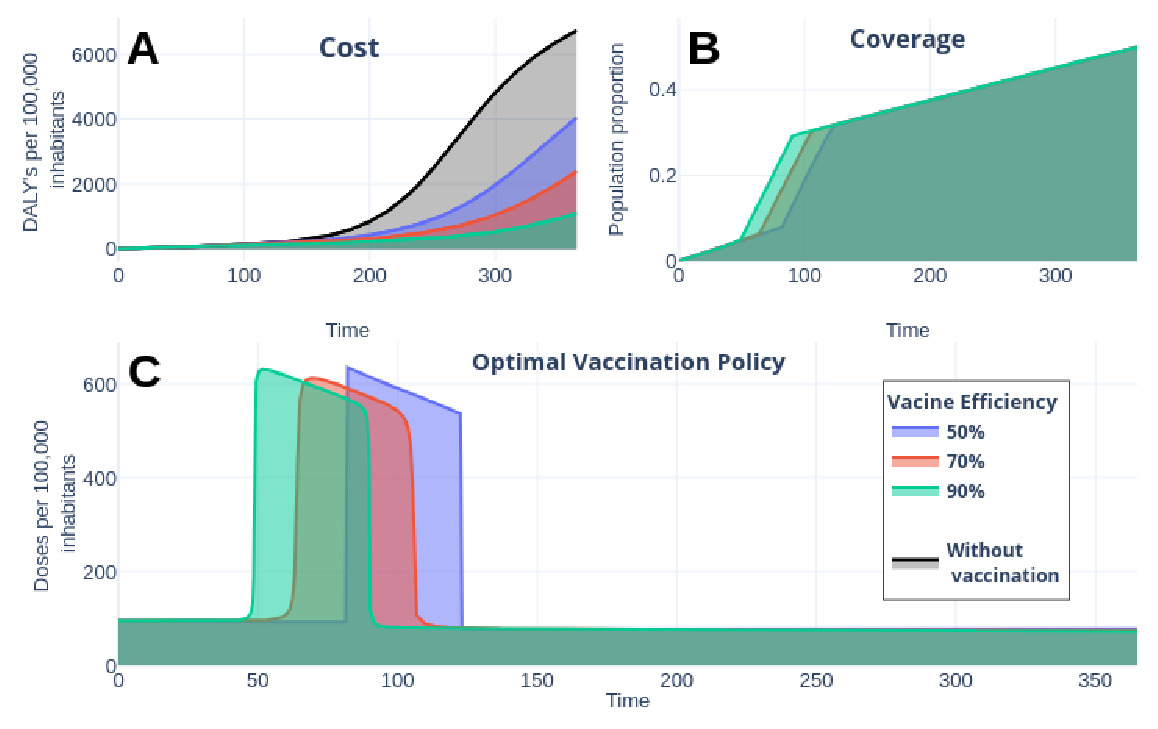
\includegraphics[scale=.60, keepaspectratio]{%
        ./EfficiencyVaccineProfile.png%
    }
    \caption[The response of COVID-19 on vaccine efficacy]{
        The response of COVID-19 burden on vaccine efficacy.
        (A) COVID-19 burden response quantified in DALYs per
        \SI{100000}{inhabitants}  to
        vaccines with efficacy of \SI{50}{\percent} (blue),
        \SI{70}{\percent} and \SI{90}{\percent}(red).
        (B) Coverage evolution to reach \SI{50}{\percent} of the total
        population vaccinated.
        (C) Optimal vaccination doses schedule according to the
        different efficacies. See
        \href{https://plotly.com/~sauldiazinfante/85/}{%
            https://plotly.com/~sauldiazinfante/85/} for
        visualization and data.
    }
    \label{fig:efficiencyvaccineprofile}
\end{figure*}
%
\begin{figure*}[htb]
    \centering
    \includegraphics[scale=.6, keepaspectratio]{%
        ./EfficiencyVaccineProfileOutbreak.png%
    }
    \caption[Optimal Vaccination Policy]{
        (A) Effect of vaccine-efficacy of
        \SI{50}{\percent} (blue), \SI{70}{\percent}
        and \SI{90}{\percent} (red) on prevalence
        of symptomatic cases per \SI{100000}{inhabitants}.
        (B) Effect of vaccine-efficacy on the number of saved lives.
        See
        \href{https://plotly.com/~sauldiazinfante/100/%
        }{https://plotly.com/~sauldiazinfante/100/} for data and
        visualization.
    }
    \label{fig:efficiencyvaccineprofileOutbreak}
\end{figure*}

\section*{Vaccine-induced immunity (SCN-3)}
Vaccine response is also strongly related to its induced immunity
\textemdash parameter that remains poorly understood
\cite{Jeyanathan2020}.
Here we contrast two vaccines with different induced immunity. Let
denote by $vax_1, vax_2$ vaccines with an induced-immunity capacity of one and
two years, respectively, and common efficacy of \SI{70}{\percent}. Consider a
vaccine camping of time horizon of one year and \SI{50}{\percent} coverage.
Taking the same dynamics parameters, that is initial conditions, and base
line parameters as in  \Cref{tbl:fixed_parameters} we explore a
contra factual scenario with an uncontrolled outbreak of
$R_0 = \num{1.79493}$ and two controlled dynamics according to vaccines
$vax_1$, $vax_2$. Thus, according to these immunity parameters and factor
defined in  \Cref{eqn:mitigation_factor},
respectively, results
$R_V^{[vax_1]} = \num{1.13913}$, $R_V^{[vax_2]} = \num{0.86756}$
for vaccine immunities periods of one and two years. We display in
\Cref{fig:induced_immunity_vaccine_profile} the response of the
vaccines $vax_1$ and $vax_2$. Since in this set time
horizon is of one year, the optimal policies follows similar schedules and
implies similar gains in the number of years of life lost. Despite this
similarities, \Cref{fig:inducedimmunity_vaccine_outbreak}
displays in panel A a dramatically gain respect to the
uncontrolled outbreak\textemdash since
$R_V ^{[vax_1]}$ is near to one, prevalence fall-down more than five times
and because $R_V ^{[vax_2]}$ is lest that one, prevalence of symptomatic
cases tends to zero with damped oscillations.
\Cref{fig:inducedimmunity_vaccine_outbreak} also endorses this gain,
note that saved lives is represented by  shaded region with translucent
and overlapped red blue colors.
%
%-------------------------------------------------------------------------------
% Induced vaccine immunity gradient
\begin{figure*}[htb]
    \centering
    \includegraphics[scale=0.6, keepaspectratio]{%
        InducedImmunityVaccineProfile%
    }
    \caption[
    Effect of Vaccine-induced immunity effect on the burden of COVID-19.
    ]{
        (A) Effect on the burden of COVID-19 quantified in DALYs per
        \SI{100000}{inhabitants} due to vaccine-induced immunity of
        \SI{365}{days}(red) and 730 days (blue).
        (B) Coverage evolution to reach \SI{50}{\percent} of the total
        population vaccinated.
        (C) Optimal vaccination doses schedule according to the different
        vaccine-induced immunities. Since the time horizon is
        \SI{350}{days}, both policies follow similar profiles in coverage
        and schedule. Visualization and data in
        \href{https://plotly.com/~sauldiazinfante/111/}{%
            https://plotly.com/~sauldiazinfante/111/}.
    }
    \label{fig:induced_immunity_vaccine_profile}
\end{figure*}
%
\begin{figure*}[htb]
    \centering
    \includegraphics[scale=0.6,keepaspectratio]{%
        InducedImmunityVaccineProfileOutbreak%
    }
    \caption[
    Effect of vaccine-induced immunity on mitigation and saved lives of
    COVID-19 outbreak]{
        (A) Effect of vaccine-induced immunity on mitigation of symptomatic
        prevalence per \SI{100000}{inhabitants}.
        (B) Number of saved lives. Since the reproductive vaccine number
        for the immunity of \SI{365}{days} results in \num{1.13913}, and
        \num{0.86756} for \SI{730}{days}, this behavior is consistent.
        See \href{https://plotly.com/~sauldiazinfante/123/}{%
            https://plotly.com/~sauldiazinfante/123/}
        for data and visualization.
    }
    \label{fig:inducedimmunity_vaccine_outbreak}
\end{figure*}
%-------------------------------------------------------------------------------
\section*{Natural Immunity Hypothesis (SCN-4)}
%
``Second infections raise questions about long-term immunity to
COVID-19 and the prospects for a vaccine'',  reported
Heidi Ledford in \cite{Ledford2020b}. Following this line, we
display in \Cref{%
    fig:natural_recovering_profile,%
    fig:natural_recovering_outbreak} the vaccine's response with
\SI{90}{\percent} efficacy and
contrasting with  natural immunity periods of
\SI{90}{days}, \SI{180}{days}, \SI{365}{days}. Here,
the adjective ``natural'' denotes the immunity that an individual
develops after recovering from a previous bout of COVID-19. When natural
immunity lasts one year, the burden of COVID-19 fall-down until around
\SI{120}{DALYs}. We confirm this behavior in the prevalence of symptomatic
cases and cumulative deaths, as displayed in
\Cref{fig:natural_recovering_outbreak}. When natural immunity is
\SI{365}{days} the gain in mitigation concerning a natural immunity of
\SI{90}{days} is at least and \num{100} times, while the number of deaths
with a natural immunity of \SI{90}{days} reach \num{845} cases per
\SI{100000}{inhabitants}, in contrast, of \SI{206} when natural immunity is
\SI{365}{days}. Thus, this simulation suggests that natural immunity
plays a vital role in the controlled outbreak's behavior, which is
consistent with the conclusions reported in \cite{Jeyanathan2020}.
%
\begin{figure*}[tbh!]
    \centering
    \includegraphics[scale=0.6,
    keepaspectratio]{NaturalRecoveringProfile}
    \caption[Effect of natural immunity on the burden of COVID-19]{
        (A) Effect on the burden of COVID-19 quantified in DALYs per
        100,000 inhabitants due to natural immunity of 90 days (red),
        180 days (yellow) and 365 days (green).
        (B) Coverage evolution to reach \SI{50}{\per} of the total
        population vaccinated.
        (C) Optimal vaccination doses schedule according to the different
        natural immunities.
        \href{https://plotly.com/~sauldiazinfante/95/}{%
            https://plotly.com/~sauldiazinfante/95/}
    }
    \label{fig:natural_recovering_profile}
\end{figure*}
%
\begin{figure*}[h!]
    \centering
    \includegraphics[scale=0.6, keepaspectratio]{%
        NaturalRecoveringProfileOutbreak%
    }
    \caption[Vaccine induced immunity profile.]{
        (A) Effect of  immunity on mitigation of
        symptomatic prevalence per 100,000 inhabitants.
        (B) Number of saved lives. Since the reproductive vaccine number
        for the immunity of 365 days results in \num{1.13913} and
        \num{0.86756} for \SI{730}{days}, this behavior is consistent.
        Plotly visualization and data in
        \href{https://plotly.com/~sauldiazinfante/104/}{%
            https://plotly.com/~sauldiazinfante/104/
        }.
    }
    \label{fig:natural_recovering_outbreak}
\end{figure*}
    \section{Conclusions and Discussions}
        
At the date of writing this article, humankind lacks strategies to
eradicate COVID-19.  Although NPIs implemented in most countries prevent
citizens from being infected, these strategies leave them
susceptible\textemdash people can not develop immunity to face futures waves.
Thus, vaccination becomes the primary pharmaceutical measure to recover life's
style before the pandemic. However, this vaccine has to be effective and well
implemented in global
vaccination programs. Thus new challenges as its distribution, stocks,
politics, vaccination efforts, among others, emerge. A fair distribution and
application strategy is imperative to manage the available resources,
especially in developing countries.

%\paragraph{Statement of principal findings}
We established an optimal control problem to design vaccination strategies
where vaccination modulates dynamics susceptibility through an imperfect
vaccine. We aimed to provide vaccination policies that minimize the lost life
years due to disability or premature death by COVID-19, determined by
cumulative deaths and cumulative incidence. Policies' acts in the minimization
of infected people's prevalence and the number of deaths.

%\paragraph{Strengths and weaknesses of the study}
Our simulations suggest a better response with optimal vaccination policies
than policies with a constant vaccination rate. For example, the optimal policy
schedule in scenario \textbf{SCN-1} increases the number of doses in the
scheme's initial stage. This vaccination scheme improves the mitigation of the
symptomatic prevalence, the incidence of deaths, and in consequence, the years
of life lost quantified in DALYs.
%

Emerging press releases reported that Pfizer's, Russian Sputnik V,
and Moderna's coronavirus vaccines reach efficacy over \SI{90}{\percent}
\cite{cnn_health_2020,reuters2020, cnn_health_2020b}. However,
this information remains under development. Thus vaccine efficacy scenarios of
\SI{50}{\percent}, \SI{70}{\percent}, and \SI{90}{\percent} \textbf{(SCN-2)}
illustrate the effect on optimal vaccination policies' schedule by pointing
when to intensify the number of doses. According to the time horizon of one
year and coverage of 50\%, our numerical experiments suggest that
\SI{90}{\percent} vaccine efficacy reduces around three times the number of
deaths regarding the dynamics without vaccination. Likewise, these vaccines
reach a gain of eighteen times in the years of life lost compared to the
without vaccination scenario.


Our numerical experiments also illustrate vaccine-induced immunity's
relation between the reproductive vaccination number $R_V$ and vaccination
policies \textbf{(SCN-3)}. Considering an outbreak with a reproductive number
$R_0$ of \num{1.794 93}, vaccine-induced immunity of \num{365} or
\SI{730}{days} implies a reduction of $R_0$\textemdash dropping its value
respectively to  \num{1.139130} and \num{.86756}.
Likewise, optimal policies linked to vaccine-induced immunities enhance
symptomatic prevalence mitigation and the number of saved lives. Moreover,
according to the initial number of deaths, the scenario without vaccination
accumulates \num{503} deads compared to \num{211} and \num{206} deads of the
underlying dynamics with vaccine-induced immunities.

%\paragraph{Strengths and weaknesses about other studies, discussing
%significant
%differences in results}
%
Barbosa et al. recently report in \cite{Barbosa2020} a simpler model about
modeling of COVID-19 vaccination with a similar approach. Although they
establish a less detailed model \textemdash they do not distinguish between
symptomatic and asymptomatic infected individuals\textemdash its control
problem return policies according to multi-objective policies. Their optimal
policy is pragmatic but, in our opinion, not necessarily practical for large
populations. Further, our model extends the result of \cite{Barbosa2020} by a
more detailed vaccine profile. Thus we can evaluate how vaccine efficacy,
vaccine-induced, and natural immunity parameters impact the mitigation of an
optimal vaccination schedule.

Perkins and España report in \cite{Perkins2020} a vaccination model with
optimal control, but they approach to optimize the NPIs. The methodology
presented here is similar, but aim very different. However, we want to stress
the relevance of also including NPIs effects.

%\paragraph{Meaning of the study: possible explanations and implications for
%clinicians and policymakers}
Since any vaccine's efficacy will be subject to uncertainty and immunization
regarding COVID-19 remains under development, policymakers need better modeling
tools to design fair vaccination programs. We faced this problem by simulation.

%\paragraph{Unanswered questions and future research}
According to DALYs definition, segregation as age, comorbidities, and other
risk groups is imperative to design more realistic vaccination policies.
Moreover, it is well-known that various vaccines platforms and strategies are
developing in parallel, and the most recent advance is with vaccines that
require two doses. From \cite{Perkins2020}, we can deduce that NPIs, together
with
vaccination, would constitute a better description of COVID-19 control. We will
direct our attention to extend this work according to the segregation and
optimization of NPIs-vaccination controls.



    \section*{Acknowledgement}
    The authors acknowledge support
    from grant DGAPA-PAPIIT IV100220
    and the Laboratorio Nacional de
    Visualización Científica UNAM.
    MAAZ acknowledges support from
    PRODEP Programme (No.
    511-6/2019-8291). DBC
    acknowledges support from PRODEP
    Programme (). We thank Jorge
    X. Velasco-Hernandez for its usefol comments and feedback.
    \section*{Author contributions}
    MAAZ .
    SDIV designed the study, provided oversight for all
    aspects of the study, developed the controlled modeling
    framework, developed simulation code for the BOCOP optimization,
    developed R-scripts for parameters calibration with Stan-R interface and
    wrote
    Sections 4 and 5 of the manuscript.
    DBC
    DOL
    \bibliographystyle{elsarticle-num-names}
    \bibliography{Vaccination_Bibliography}
    \begin{appendices}
        \section{Parameter estimation}
        \label{App:Parameter_Est}
Mathematical models for COVID-19 have shown that the
parameters' values are not necessarily the same in each country. We
use COVID-19 data from Mexico City plus Mexico state to follow the
epidemic curve's initial growth in this work. Consequently, we
estimate some parameter values of system in \Cref{model1}
\cite{DataMX}. To obtain the baseline parameter values, we consider
two-stages: i) before and ii) after mitigation measures were
implemented. For both stages, we use model in \Cref{model1} with no
vaccination dynamics ($\lambda_V = 0$ and $V(0) = 0$), and STAN
R-package. This package is used for statistical inference by the
Bayesian approach. For the code implementation of our system, we
follow ideas of \cite{Chatzilena2019}, and it is made freely available
at \cite{gitHub}. For this section, our estimations are focused on
three parameters: $\beta_A$, $\beta_S$ and $p$. Other parameter values
are given in \Cref{table_fixparam}.
\begin{table}[h!]
\begin{center}
	\begin{tabular}{ccc}
		\toprule
		Parameter & Value & References
		\\
		\midrule
		$\delta_{E}^{-1}$ & $5.1\ \text{days}$   &  \cite{Tian2020}
		\\
		$\alpha_{S}^{-1}$  & $5.97\ \text{days}$  &  \cite{Acuna2020}
		\\
		$\alpha_{A}^{-1}$ & $10.81\ \text{days}$ & \cite{Acuna2020}
		\\
		$\delta_{R}^{-1}$ & $365\ \text{days}$     &
		\\
		$\mu^{-1}$        & $70\ \text{years}$   &
		\\
		\bottomrule
		\end{tabular}
		\caption{Fixed parameters values of system in
		\Cref{model1}.}\label{table_fixparam}
	\end{center}
\end{table}

For the first stage, the following system is considered:
\begin{equation}\label{model_stage1}
  \begin{aligned}
	S'(t)&=\mu \bar{N}-\frac{\hat{\beta}_S
	I_S+\hat{\beta}_AI_A}{\bar{N}}S-\mu S + \delta_R R\\
	E'(t)&= \frac{\hat{\beta}_S I_S+\hat{\beta}_A
	I_A}{\bar{N}}S-(\mu+\delta_E) E \\
	I'_S(t)&= p \delta_E E-(\mu+\alpha_S) I_S\\
	I'_A(t)&= (1-p) \delta_E E-(\mu+\alpha_A) I_A \\
	R'(t)&= (1-\theta) \alpha_S I_S+\alpha_A I_A-(\mu+\delta_R) R \\
	D'(t)&= \theta \alpha_S I_S
  \end{aligned}
\end{equation}
where $\bar{N}(t)=S(t)+E(t)+I_S(t)+I_A(t)+R(t)$ and $N=\bar{N}+D$.
Here, we consider COVID-19 data from the first day of symptoms onset
reported (February 19) until March 23, 2020. We also assume that
$\theta = 0$ because the first reported death was on March 18, and
there were three reported deaths until March 23. The initial values of
recovered and dead people are set to zero. Symptomatic class initial
value was fixed in one individual, while $E(0)$ and $I_{A}(0)$ were
estimated. Thus, $S(0) = N - (E(0) + I_{A}(0) + 1)$, where $N =
26446435$ \cite{conavi2020}. For the STAN implementation, we employ a
negative-binomial model as the likelihood function with the mean
parameter given by incidence solution per day. In addition to the
above, we assign prior probability distributions to each parameter and
the exposed and asymptomatic classes' initial conditions. Thus, we
propose that $\hat{\beta}_A$ and $\hat{\beta}_S$ follow a normal
distribution with parameters $\mu = 1$ and $\sigma^2 = 0.13$. Then,
$p$ follows a uniform distribution in $(0, 0.25)$, and $E(0)$ and
$I_{A}(0)$ also follow a uniform distribution in $(2,20)$ and
$(2,10)$, respectively. When employing our STAN implementation, we run
5 chains with 100,500 iterations each, discard the first 500, and use
10,000 samples to generate estimates of parameters $\hat{\beta}_A$,
$\hat{\beta}_S$ and $p$. \Cref{table_icparam} shows the confidence
interval for each parameter and median posterior estimated.
\begin{table}[h!]
\begin{center}
	\begin{tabular}{ccc}
		\toprule
	    Parameter & 95\% Confidence Interval & Quantile 50
			\\
			\midrule
            $\hat{\beta}_S$ & $[0.672, 1.1886]$   &  $0.9322$ \\
            $\hat{\beta}_A$ & $[0.501, 0.7851]$  &  $0.6435$ \\
            $p$       & $[0.061, 0.2206]$ &  $0.1227$ \\
            $R_0$ & $[4.159, 5.1991]$ &  $4.6082$ \\
			\bottomrule
	\end{tabular}
  \caption{Confidence interval and median posterior estimated for some
  parameters of system in \Cref{model_stage1} and basic reproductive
  number $(R_0)$.}\label{table_icparam}
\end{center}
\end{table}

\noindent For the second stage, we took a complete month starting the
day when mitigation measures were implemented, that is, from March 23
to April 23, 2020. Now, we consider parameter $\xi$ to model the
implementation of non-pharmaceutical measures. Thus, system in
\Cref{model_stage1} becomes:
\begin{equation}\label{model_stage2}
  \begin{aligned}
	S'(t)&=\mu \bar{N}-\frac{\xi\hat{\beta}_S
	I_S+\xi\hat{\beta}_AI_A}{\bar{N}}S-\mu S + \delta_R R\\
	E'(t)&= \frac{\xi\hat{\beta}_S
	I_S+\xi\hat{\beta}_AI_A}{\bar{N}}S-(\mu+\delta_E) E \\
	I'_S(t)&= p \delta_E E-(\mu+\alpha_S) I_S\\
	I'_A(t)&= (1-p) \delta_E E-(\mu+\alpha_A) I_A \\
	R'(t)&= (1-\theta) \alpha_S I_S+\alpha_A I_A-(\mu+\delta_R) R \\
	D'(t)&= \theta \alpha_S I_S
  \end{aligned}
\end{equation}
where $\bar{N}(t)=S(t)+E(t)+I_S(t)+I_A(t)+R(t)$ and $N=\bar{N}+D$. At
this stage, we consider that $\theta = 0.11$. Here, our objective is
to estimate the value of parameter $\xi$. To do this, we use the
median posterior of all the estimated parameters from the first stage
(see \Cref{table_icparam}). Other parameter values are given in
\Cref{table_fixparam}. Almost all initial conditions were obtained
when solving system in \Cref{model_stage1} with the 10,000 samples
(obtained in first stage), after which each solution at the final time
(March 23) is saved. We use the median of the saved values. Thus, for
system in \Cref{model_stage2}, $E(0) = 6587.585$, $I_S(0) = 553.7035$,
$I_A(0) = 3149.924$, and $R(0) = 3001.547$. For the initial value of
variable $D$, we consider reported COVID-19 data, then $D(0) = 3$.
Therefore $S(0) = N - (E(0) + I_S(0) + I_A(0) + R(0) + D(0))$, with $N
= 26446435$ \cite{conavi2020}. Similar to the first stage, we consider
a negative-binomial model as the likelihood function with the mean
parameter given by incidence solution per day, while that we postulate
a uniform distribution in $(0.25,0.75)$ as a prior probability
distribution for the parameter $\xi$.
%\label{App:Parameter_Est}
For the second stage, we run 5 chains with 100,500 iterations each,
discard the first 500, and use 10,000 samples to generate estimates of
parameters $\xi$. \Cref{table_icparam2} shows the confidence interval
and median posterior estimated for parameter $\xi$.
\begin{table}[h!]
\begin{center}
	\begin{tabular}{ccc}
		\toprule
	    Parameter & 95\% Confidence Interval & Quantile 50
			\\
			\midrule
            $\xi$     & $[0.3696, 0.4099]$  & $0.3889$  \\
            $R_0$ & $[1.702, 1.887]$ &  $1.791$ \\
			\bottomrule
	\end{tabular}
  \caption{Confidence interval and median posterior estimated for
  parameter $\xi$ of system in \Cref{model_stage2} and basic
  reproductive number $(R_0)$.}\label{table_icparam2}
\end{center}
\end{table}

Finally, it is important to mention that our results were implemented
considering that the effective transmission contact rates
$(\beta_{\bullet})$ were equal to $\xi\hat{\beta}_{\bullet}$. This
last means that our scenarios consider the first reduction in the
effective transmission contact rates by NIPs. Using values in
\Cref{table_icparam,table_icparam2}, we build confidence intervals for
$\xi\hat{\beta}_{\bullet}$. These results are shown in
\Cref{table_icparam3}.
\begin{table}[h!]
\begin{center}
	\begin{tabular}{cc}
		\toprule
	    Parameter & 95\% Confidence Interval
			\\
			\midrule
            $\beta_S = \xi\hat{\beta}_S$ & $[0.2483712, 0.48720714]$ \\
            $\beta_A = \xi\hat{\beta}_A$ & $[0.1851696, 0.32181249]$ \\
			\bottomrule
	\end{tabular}
  \caption{Confidence interval for parameters
  $\beta_{\bullet}$.}\label{table_icparam3}
\end{center}
\end{table}

    \end{appendices}
\end{document}
